\documentclass[conference]{IEEEtran}
\usepackage{amsmath,amssymb,booktabs,graphicx,url}
\usepackage[hidelinks]{hyperref}
\usepackage{tikz}\usetikzlibrary{arrows.meta,positioning}
\begin{document}
\title{Leak-Free Fine-Tuning of a Phase-Aware Enhancer and Diagnosing Test-Set Mismatch for Indic Noise-Event Removal}
\author{\IEEEauthorblockN{Avinash Kumar Sharma (Team Vedanga)}
\IEEEauthorblockA{Wadhwani School of Data Science and AI, IIT Madras, Chennai, India\\ avics2020@gmail.com}}
\maketitle

\begin{abstract}
We describe our solution to Track~2 (Noise Event Removal) of Datathon@IndoML 2026, scored as SI-SDR on synthetic clips plus $100\times\Delta$WER of the mandated SraVaani-1.0 ASR. We fine-tune the phase-aware MP-SENet (2.26\,M parameters), initialised from its DNS-Challenge checkpoint, in four warm-started stages on simulated Vaani mixtures built with a leak-free protocol: validation noise events are clustered and only training clusters are used, because 98.8\% of the validation events are reused across clips. Inference uses 8-s windows and shift test-time augmentation (TTA). The selected submission scores 15.21 (SI-SDR 13.18\,dB, $\Delta$WER $+2.02$\%). We also diagnose why local and leaderboard scores differ by about 5\,dB: test clips are three times longer, mostly event-free, and their references keep native Vaani noise. A local set built from noisy Vaani clips plus unseen library events reproduces the leaderboard SI-SDR of our model (12.66 vs.\ 13.18\,dB), and an ``event-only'' training recipe improves it by 0.28\,dB.
\end{abstract}

\section{Introduction}
Track~2 asks for 16-kHz enhanced audio that suppresses noise events (horns, animals, appliances, alarms, etc.) in spontaneous Indic speech while preserving the speech. Submissions are scored as $\text{Combined}=\text{SI-SDR}_\text{syn}+100\,\Delta\text{WER}$, where SI-SDR~\cite{sisdr} is averaged over the 1{,}099 synthetic test clips and $\Delta$WER is the pooled WER reduction of SraVaani-1.0 over all 3{,}178 test clips (1{,}099 synthetic, 2{,}079 natural); transcripts are audited by re-running the ASR on the submitted WAVs. The test set provides audio only (no timestamps). Our solution has three parts: a leak-free validation protocol, staged fine-tuning of a phase-aware enhancer on Vaani-like simulations, and an inference recipe tuned for long clips. We also report what failed and a diagnosis of the local/leaderboard gap.

\section{Training Data and Preprocessing}
\textbf{Vaani.} Clean speech comes from the Gold split of ARTPARK-IISc/Vaani-Noise-Event-Dataset~\cite{vaani}: event-free spans ($\ge$2.5\,s) carved with the organisers' baseline~\cite{baseline} from 6{,}000 clips (3{,}968 spans, early stages) and 11{,}000 clips (8{,}733 spans, final stages).

\textbf{Validation and leak-free split.} The validation set has 695 synthetic pairs (noisy, clean reference, timestamps) and 1{,}806 natural clips. Noise events are isolated as noisy$-$clean inside the timestamps (1{,}819 events). Near-duplicates are clustered (cosine $>0.95$ on 48$\times$48 log-mel fingerprints; 139 clusters) and 62 clusters are held out; the 228 synthetic clips whose events all lie in held-out clusters form the evaluation set, and only the 644 events of training clusters enter the noise bank. A first model fine-tuned on a random validation split scored 12.3\,dB locally but 0.83 on the leaderboard, which exposed the reuse.

\textbf{Additional data.} ESC-50~\cite{esc50} (1{,}998 trimmed event segments, $\le$2.5\,s; CC BY-NC 3.0) and the MUSAN noise subset~\cite{musan} (930 files $\rightarrow$ 2{,}456 random crops of 0.5--2.5\,s; CC BY 4.0).

\textbf{Augmentation.} One augmented copy per noise segment: speed 0.9/1.0/1.1; with $p{=}0.6$ a 4th-order low-pass (2--7\,kHz) or 2nd-order high-pass (100--500\,Hz); with $p{=}0.5$ a synthetic exponentially decaying reverb (RT 0.15--0.7\,s). Final pool: 10{,}192 segments.

\textbf{Mixing.} 5-s mixtures with 1--4 events of 0.3--2.5\,s at event SNR $\in[-20,5]$\,dB relative to speech (mean input SI-SDR $\approx-5$\,dB), matching the validation statistics. Datasets: 8k (stage 1), 16k (stage 2) and 40k mixtures (stages 3--4).

\section{Proposed Method}
\textbf{Architecture.} MP-SENet~\cite{mpsenet} predicts magnitude and phase in parallel from the compressed STFT ($n_\text{fft}{=}400$, hop 100, compression 0.3) with four time--frequency Transformer blocks. We keep the official configuration and initialise from the DNS-Challenge~\cite{dns} checkpoint \texttt{g\_best\_dns}. Replacing the baseline magnitude-mask BiGRU (noisy phase) by this phase-aware model was the largest single gain (3.40 $\rightarrow$ 10.00 zero-shot).

\textbf{Loss.} Generator terms of MP-SENet without the metric discriminator: $\mathcal{L}=0.9\,\mathcal{L}_\text{mag}+0.3(\mathcal{L}_\text{IP}+\mathcal{L}_\text{GD}+\mathcal{L}_\text{IAF})+0.2\,\mathcal{L}_\text{com}+0.2\,\mathcal{L}_\text{con}+0.2\,\mathcal{L}_\text{time}$ (MSE on compressed magnitude and complex spectra, anti-wrapping phase losses, STFT consistency, waveform L1). An ASR-feature loss on SraVaani encoder features helped the small baseline (+0.8) but on MP-SENet traded SI-SDR for ASR roughly one-to-one ($\lambda{=}0.5$/1.5) and was not used.

\textbf{Training.} AdamW~\cite{adamw} ($\beta{=}0.8/0.99$), OneCycle~\cite{onecycle} (5\% warm-up), gradient clipping 5, inputs RMS-normalised. Stage 1 (E8): DNS init, LR $2{\times}10^{-4}$, 5 epochs, 1-s crops, batch 2, fp32 on a T4 (fp16 AMP silently skipped updates). Stage 2 (E9-B): LR $10^{-4}$, 3 epochs, 16k mixtures. Stage 3: 40k mixtures, 3-s crops, batch 4, bf16 forward on an A100; the 8-epoch schedule did not decay within the time budget (held-out 17.00\,dB). Stage 4 (annealing): one epoch (9{,}500 steps) with LR $5{\times}10^{-5}$ decaying to $\approx0$ gives model D (17.26\,dB). Lesson: size the schedule to the measured throughput.

\textbf{Reproducibility.} Training and inference code, configuration files, the final checkpoint and the original notebooks are released in our public repository; the README lists the software and hardware (A100-SXM4 80\,GB with PyTorch 2.8/CUDA 12.8 for the final stages and inference; Kaggle T4 for early stages).

\textbf{Inference.} Each clip is RMS-normalised and enhanced on 8-s windows (6-s hop, linear cross-fades); 60\% of clips exceed 4\,s, and 8-s windows beat 4-s ones. Shift TTA averages the realigned outputs of 8 copies delayed by 0--87 samples (sub-hop STFT alignments), which reduces artefacts. Outputs are rescaled to the input RMS. Transcripts come from SraVaani-1.0~\cite{sravaani}. Every clip is processed by the model.


\begin{figure}[t]\centering
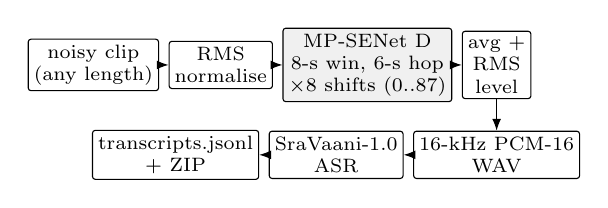
\begin{tikzpicture}[node distance=1.2mm, every node/.style={font=\scriptsize, align=center}, box/.style={draw, rounded corners=1pt, inner sep=2pt, minimum height=6mm}, ->/.style={-{Latex[length=1.5mm]}}]
\node[box] (a) {noisy clip\\(any length)};
\node[box, right=of a] (b) {RMS\\normalise};
\node[box, right=of b, fill=gray!12] (c) {MP-SENet D\\8-s win, 6-s hop\\$\times$8 shifts (0..87)};
\node[box, right=of c] (d) {avg +\\RMS\\level};
\node[box, below=4mm of d] (e) {16-kHz PCM-16\\WAV};
\node[box, left=of e] (f) {SraVaani-1.0\\ASR};
\node[box, left=of f] (g) {transcripts.jsonl\\+ ZIP};
\draw[->] (a)--(b); \draw[->] (b)--(c); \draw[->] (c)--(d); \draw[->] (d)--(e); \draw[->] (e)--(f); \draw[->] (f)--(g);
\end{tikzpicture}
\caption{Inference pipeline of the selected submission (every clip is processed by the model).}\label{fig:pipe}
\end{figure}

\begin{table}[t]\centering\caption{Training stages of the submitted model D (all warm-started; T4 fp32, A100 bf16).}\label{tab:stages}\footnotesize\setlength{\tabcolsep}{2.5pt}
\begin{tabular}{lllccc}\toprule
Stage & Init & Mix & Crop$\times$bs & LR & Held-out\\\midrule
E8 (T4) & DNS & 8k & 1\,s$\times$2 & $2{\times}10^{-4}$ & 16.68\\
E9-B (T4) & E8 & 16k+aug & 1\,s$\times$2 & $10^{-4}$ & 16.93\\
E10-R (A100) & E9-B & 40k & 3\,s$\times$4 & $10^{-4}$ & 17.00\\
Anneal$\rightarrow$D & E10-R & 40k & 3\,s$\times$4 & $5{\times}10^{-5}\!\rightarrow\!0$ & 17.26\\\bottomrule
\end{tabular}\end{table}

\textbf{Novelty: test-set diagnosis and event-only training.} Running D on 800 test clips (analysis only) showed median length 11.9\,s (validation 4.4\,s) and loud-noise occupancy of 10\% of frames (validation synthetic 39\%), while keeping the input where D removes little \emph{lowered} the test SI-SDR. A local set of \emph{noisy} Vaani clips plus unseen library events (ESC-50 fold 5, held-out MUSAN), with the Vaani clip itself as target, reproduces D's leaderboard SI-SDR (12.66 vs.\ 13.18\,dB) and its ASR pattern ($\Delta$WER $+5.1$ of a $+12.0$ ceiling, cf.\ leaderboard $+5.7$ vs.\ leaders' $\approx$17). This supports reading the task as removing only the added events while keeping native audio. We trained E13 accordingly (target = natural clip as-is, input = target + 1--3 library events; 30k mixtures from 10{,}206 natural clips; 6-s crops, 13{,}775 steps sized from a measured 5{,}009 steps/h).


\textbf{What did not help.} Detect-and-suppress gating with ground-truth timestamps on the baseline (oracle) removed speech under events; bootstrapping noise from Vaani recordings ($x-D(x)$ inside annotated events) lowered held-out scores; time-reversal TTA was worse than shift TTA at equal compute; an output high-pass filter and soft limiting reduced SI-SDR by 2--6\,dB; mixing the input back (observation adding) raised ASR but cost more SI-SDR; averaging D with zero-shot MossFormerGAN, FRCRN or MossFormer2 lowered the local score; training D to remove continuous background (E12) lost 2.7\,dB on held-out clips.

\section{Results and Conclusion}
Table~\ref{tab:lb} lists leaderboard submissions; Table~\ref{tab:local} summarises local evidence (``val'' = 228 held-out synthetic + 600 natural clips).

\begin{table}[t]\centering\caption{Codabench Phase-2 submissions.}\label{tab:lb}\footnotesize\setlength{\tabcolsep}{2.5pt}
\begin{tabular}{lccc}\toprule
Submission & SI-SDR & $\Delta$WER s/n (\%) & Comb.\\\midrule
Baseline mask-net, real.\ sim. & -- & -- & 3.40\\
MP-SENet DNS, zero-shot & -- & -- & 10.00\\
MP-SENet fine-tuned (E8) & 12.37 & 4.65 / 0.20 & 13.99\\
avg(E9-A, E9-B) & 12.73 & 5.05 / 0.27 & 14.53\\
B+D, 4-s windows & 12.86 & 5.41 / 0.31 & 14.81\\
D, 8-s + TTA$\times$4 & 13.15 & 5.69 / 0.30 & 15.18\\
\textbf{D, 8-s + TTA$\times$8} & \textbf{13.18} & \textbf{5.68 / 0.30} & \textbf{15.21}\\
D TTA$\times$8 + peak 0.95 & 13.18 & 5.09 / 0.38 & 15.07\\
D TTA$\times$8 + resid.\ gate & 12.51 & 5.26 / 0.26 & 14.37\\\bottomrule
\end{tabular}\end{table}

\begin{table}[t]\centering\caption{Local evaluations (win8 + TTA$\times$2 unless noted).}\label{tab:local}\footnotesize\setlength{\tabcolsep}{2.5pt}
\begin{tabular}{lcc}\toprule
Setting & D & alt.\\\midrule
val comb.: win4 vs win8+TTA$\times$8 & 18.44 & 19.83\\
val comb.: +MossFormerGAN / +FRCRN & 19.20 & 17.62 / 18.53\\
held-out SI-SDR: E12 (bg.\ removal) & 17.25 & 14.57\\
natural+events SI-SDR: E13 & 15.41 & 15.82\\
12-s natural+events SI-SDR: E13 & 16.06 & 17.50\\
\textbf{noisy Vaani+events: E13} & \textbf{12.66} & \textbf{12.95}\\\bottomrule
\end{tabular}\end{table}

\textbf{Findings.} (i) Leak-free validation is essential with reused noise. (ii) The phase-aware model class and in-domain fine-tuning give most of the gain; large generic SE models are 3--5\,dB behind and hurt SraVaani. (iii) Shift TTA transfers to the leaderboard (+0.37) but only about a third of its local gain; output post-processing (loudness, gating) gains locally and loses on the leaderboard, consistent with the literature that SE artefacts, not residual noise, drive ASR errors~\cite{iwamoto}. (iv) Validation and test synthetic data differ in length and in whether native noise remains in the reference; the noisy-Vaani set is the first local evaluation that reproduces our leaderboard SI-SDR.

\textbf{Conclusion.} A small phase-aware enhancer fine-tuned on leak-free, Vaani-like simulations with budget-sized annealing and shift TTA reaches 15.21. The diagnosed test structure suggests that event-only targets on long, noisy natural clips are the next lever; E13 improves the test-mimicking set by 0.28\,dB but could not be scored on the leaderboard before the deadline.

\begin{thebibliography}{99}\footnotesize
\bibitem{mpsenet} Y.-X. Lu, Y. Ai, and Z.-H. Ling, ``MP-SENet: A speech enhancement model with parallel denoising of magnitude and phase spectra,'' in \emph{Proc. Interspeech}, 2023. Code/checkpoint: \url{https://github.com/yxlu-0102/MP-SENet}.
\bibitem{dns} C. K. A. Reddy \emph{et al.}, ``The INTERSPEECH 2020 Deep Noise Suppression Challenge: Datasets, subjective testing framework, and challenge results,'' in \emph{Proc. Interspeech}, 2020.
\bibitem{vaani} ARTPARK-IISc, ``VAANI Noise Event Dataset: A curated spontaneous speech dataset annotated with timestamps for noise events,'' arXiv:2609.02474, 2026.
\bibitem{sravaani} ARTPARK-IISc, ``SraVaani-1.0,'' \url{https://huggingface.co/ARTPARK-IISc/SraVaani-1.0}.
\bibitem{baseline} S. Nag \emph{et al.}, ``noise-event-detection-and-removal (IndoML 2026 baseline),'' \url{https://github.com/nagshubhadip/noise-event-detection-and-removal}.
\bibitem{esc50} K. J. Piczak, ``ESC: Dataset for environmental sound classification,'' in \emph{Proc. ACM Multimedia}, 2015.
\bibitem{musan} D. Snyder, G. Chen, and D. Povey, ``MUSAN: A music, speech, and noise corpus,'' arXiv:1510.08484, 2015.
\bibitem{sisdr} J. Le Roux, S. Wisdom, H. Erdogan, and J. R. Hershey, ``SDR -- half-baked or well done?'' in \emph{Proc. ICASSP}, 2019.
\bibitem{iwamoto} K. Iwamoto \emph{et al.}, ``How bad are artifacts?: Analyzing the impact of speech enhancement errors on ASR,'' in \emph{Proc. Interspeech}, 2022.
\bibitem{adamw} I. Loshchilov and F. Hutter, ``Decoupled weight decay regularization,'' in \emph{Proc. ICLR}, 2019.
\bibitem{onecycle} L. N. Smith and N. Topin, ``Super-convergence: Very fast training of neural networks using large learning rates,'' in \emph{Proc. SPIE}, 2019.
\end{thebibliography}
\end{document}
